\chapter{ESTRUTURA DE APOIO}

%Adicionar introdução do capítulo

\section{ATIVIDADES DE TUTORIA}

As atividades de tutoria são parte fundamental na melhoria do processo de acompanhamento dos discentes, seja no início do curso, com atividades de acolhimento e ambientação, seja durante o curso, nas atividades das disciplinas semipresenciais e não presenciais.

No contexto do curso de Engenharia Eletrônica existem vários grupos estudantis que atuam no processo de ambientação, acolhimento e tutoria dos discentes ingressantes. Estes grupos estudantis são acompanhados por docentes na execução das atividades com os discentes ingressantes. Atualmente, fazem parte destas atividades:

\begin{itemize}
    \item Centro Acadêmico de Engenharia Eletrônica (\href{facebook.com/caee.utf.td}{CAEE});
    \item Equipe \href{facebook.com/hefestus.utfpr}{Hefestus} de Robótica;
    \item Empresa Júnior \href{exata.org.br}{EXATA}.
\end{itemize}
    
A partir da reformulação deste PPC, disciplinas semipresenciais e não presenciais passam a compor a matriz curricular do curso. Desta forma, a Resolução 39/2019  (!!Referenciar) regulamenta a criação e a oferta de unidades curriculares na modalidade semipresencial e na modalidade não presencial, em cursos de Graduação presenciais da UTFPR. Conforme o previsto nessa resolução, será definida uma metodologia de tutoria presencial e não presencial pelos docentes e por monitores discentes preparados para este fim.

\section{TECNOLOGIAS DE INFORMAÇÃO E COMUNICAÇÃO (TIC) NO PROCESSO ENSINO-APRENDIZAGEM}
\label{sec:tic}

% Os mecanismos de interação são caracterizados como 

% \begin{citacao}
%     ``o conjunto de estruturas de Tecnologia de Informação e Comunicação (TIC) e os respectivos procedimentos e as formas de utilização que caracterizam a dinâmica da comunicação e da interação entre os sujeitos envolvidos nos processos acadêmicos e de ensino e aprendizagem (que são, basicamente, os docentes, tutores e discentes), no contexto da oferta do curso superior na modalidade à distância'' (BRASIL, 2004) (!! Referenciar - vem do ppc atual).
% \end{citacao}

De acordo com o Instrumento de Avaliação de Curso de 2017 \cite{instrumento2017}, as tecnologias da informação e da comunicação (TIC) são: 

\begin{citacao}
    ``Recursos didáticos constituídos por diferentes mídias e tecnologias, síncronas e assíncronas, tais como: ambientes virtuais e suas ferramentas; redes sociais e suas ferramentas; fóruns eletrônicos; blogs; chats; tecnologias de telefonia; teleconferências; videoconferências; TV; rádio; programas específicos de computadores (\textit{softwares}); objetos de aprendizagem;   conteúdos disponibilizados em suportes tradicionais ou em suportes eletrônicos''.
\end{citacao}

O uso de recursos tecnológicos aplicados à educação e comunicação é importante enquanto podem ilustrar conceitos abstratos complexos e enriquecer o contexto de ensino e aprendizagem. Nesse cenário, complementar as técnicas tradicionais com elementos que facilitem a assimilação dos assuntos abordados e contribuam para que a interação entre alunos e professores se torne mais interessante e produtiva pode representar o diferencial em cursos que exijam alto grau de abstração.

As ferramentas de Tecnologia de Informação e Comunicação (TIC) incluem desde conteúdos digitais bem preparados, que podem ser facilmente disponibilizados, passando pela manutenção de sítios \textit{online}, que se tornam repositórios de informação, chegando a mecanismos mais elaborados de gerenciamento de conteúdo e colaboração.

Os mecanismos de interação são caracterizados como o conjunto de estruturas de Tecnologia de Informação e Comunicação (TIC) e os respectivos procedimentos e as formas de utilização que caracterizam a dinâmica da comunicação e da interação entre os sujeitos envolvidos nos processos acadêmicos e de ensino e aprendizagem (que são, basicamente, os docentes, tutores e discentes), no contexto da oferta do curso superior na modalidade a distância \cite{instrumento2017}.

%[77] Universidade Tecnológica Federal do Paraná, “Deliberação COUNI nº 13/2009 - Atualização Regulamento CPA,” Curitiba, 2009.
%[78] Ministério da Educação, “Instrumento de Avaliação de Cursos de Graduação - 2012,” Brasília, 2012.


A instituição disponibiliza alguns ambientes e artefatos de comunicação para mediarem atividades didáticas nas modalidades presencial e não presencial:

\begin{itemize}
    \item Página pessoal docente;
    \item Moodle institucional;
    \item Plataforma GSuite for Education;
    \item Serviço Mconf em parceria com a Rede Nacional de Ensino e Pesquisa (RNP);
    \item Base Digital de dados;
    \item Repositórios institucionais;
    \item Office 365;
    \item Equipamentos de áudio e vídeo em geral.
\end{itemize}
    
Diante disso, o processo de ensino aprendizagem é intensificado com o uso das TIC e demais artefatos tecnológicos, por meio de atividades de comunicação, colaboração e compartilhamento, propiciando a construção e a produção de conhecimentos e o desenvolvimento de habilidades pessoais e interpessoais do corpo discente, e fomentando novas práticas do docente.

Os recursos tecnológicos disponíveis no campus são mediados pela Coordenação de Gestão de Tecnologia da Informação (COGETI), sendo responsável pelo Moodle institucional. Adicionalmente, dá suporte à infraestrutura de redes, manutenção de computadores e instalação de \textit{softwares}. Além disso, o sistema de bibliotecas disponibiliza ampla base digital de dados e repositórios institucionais para produção acadêmica em geral.

As salas de aula da UTFPR, campus Toledo, são equipadas com projetor multimídia, o que facilita a utilização de objetos educacionais digitais por parte do professor, tais como a exibição de slides e vídeos. Além disso, um espaço para disponibilização de conteúdo está disponível para utilização dos docentes (páginas pessoais), por meio da criação facilitada de páginas que ficam armazenadas em servidores próprios da instituição. Tais páginas podem conter arquivos, endereços de Internet (\textit{hyperlinks}), imagens, notícias.

O Moodle é um ambiente de suporte à aprendizagem que possui diversos recursos relacionados ao gerenciamento de conteúdo e trabalho colaborativo, como questionários, tarefas, glossários, fóruns e salas de conversação. Considerando estas possibilidades e a infinidade de material educacional de boa qualidade que pode ser obtido e disponibilizado via Internet, tem-se ampliadas as oportunidades de enriquecimento e facilitação da aprendizagem.

É importante ressaltar que a instituição tem oferecido continuamente cursos de capacitação do ambiente Moodle, em semanas de planejamento didático pedagógico, para que os professores possam conhecer a plataforma e aproveitar o máximo dos recursos disponíveis em prol da melhoria do ensino.

A instituição mantém ainda uma página web do curso na qual são disponibilizadas informações para os alunos sobre a estrutura curricular, docentes e infraestrutura, entre outros.

Além da utilização das TIC no curso, a UTFPR promove o desenvolvimento de TIC para os alunos com auxílio financeiro. Os alunos, acompanhados de um professor orientador, elaboram um projeto que, se aprovado pelo órgão avaliador, passa a desenvolver a tecnologia para ser aplicada na própria instituição.


\section{AMBIENTES DE APRENDIZAGEM}
\label{sec:amb}

Com relação à infraestrutura dos ambientes de ensino e aprendizagem, atualmente o campus dispõe de:

\begin{itemize}
    \item 18 salas de aula com capacidade para 50 alunos cada, sendo que estas são equipadas com projetor multimídia, ventiladores e quadro branco e 2 salas com capacidade de 24 alunos com os mesmos equipamentos listados anteriormente;
    \item Uma sala de atendimento de monitoria;
    \item Uma sala de estudo 24 horas;
    \item Sete laboratórios de informática para aulas teóricas ou práticas que necessitem de \textit{softwares};
    \item Seis laboratórios de exclusivos para os alunos do curso de Engenharia Eletrônica;
    \item Dois laboratórios de aulas práticas de Física;
    \item Sete laboratórios para aulas práticas de química com capacidade para 24 alunos cada;
    \item Uma biblioteca, com 5 salas de estudo, mesas de estudos individuais, livros da bibliográfica básica e complementar (entre outros), revistas, periódicos, computadores com acesso a rede e equipado com os \textit{softwares} utilizados em nos laboratórios de informática.
\end{itemize}

Já em termos de ambientes virtuais de aprendizagem (já citados na \autoref{sec:tic}), estes devem proporcionar a discente e docente recursos que facilitem a execução de atividades síncronas e assíncronas, bem como meios para interação e devolutiva ao discente. Atualmente, a UTFPR disponibiliza ao menos dois ambientes virtuais principais de ensino aprendizagem (AVEA): Moodle e \textit{Gsuit for Education}.

O ambiente Moodle é uma ferramenta já amplamente empregada em disciplinas presenciais, semipresenciais e não presenciais. Trata-se de um sistema de gerenciamento de aprendizagem \textit{open-source} e gratuito. Pode ser utilizado para diversos fins educacionais, seja na educação a distância, organização de materiais educacionais e auxílio a metodologias ativas.

O ambiente \textit{Gsuit for Education} é uma plataforma educativa colaborativa, que une diversos recursos disponíveis do Google. Nesta plataforma é possível utilizar editor de texto, apresentação de slides, planilhas, agenda, e drive, todos de forma colaborativa. Além disso, o Google \textit{Classroom} auxilia no gerenciamento de uma sala virtual e encontros síncronos podem ocorrer com a ferramenta Google \textit{Meet}.

\section{MATERIAL DIDÁTICO}

A respeito de materiais didáticos, há uma ampla gama de materiais que podem ser aplicados às disciplinas presenciais, semipresenciais e/ou não presenciais. Gravação de aulas, tutoriais, apostilas, guias práticos são recursos que cada professor utiliza/desenvolve, de acordo com a necessidade, para sua disciplina. Estes materiais são mantidos em repositório próprio do professor, tal como página pessoal, Moodle, Google Drive, Youtube e demais plataformas disponíveis.

Além disso, o sistema de bibliotecas disponibiliza ampla base digital de dados e repositórios institucionais para uso didático em geral.

\section{INFRAESTRUTURA DE APOIO ACADÊMICO}

A estrutura de apoio é entendida por apoio pedagógico e infraestrutura física de apoio acadêmico, de ensino e de aprendizagem.

Em termos de estrutura de apoio pedagógico, a UTFPR conta com o Departamento de Educação (DEPED) voltado à consolidação e melhoria do processo de ensino aprendizagem, conforme estabelece o Regimento Geral da UTFPR.

O DEPED é composto por:

\begin{itemize}
    \item Núcleo de Ensino (NUENS) voltado à gestão pedagógica e o atendimento direto aos docentes;
    \item Núcleo de Acompanhamento Psicopedagógico e Assistência Estudantil (NUAPE) voltado ao atendimento coletivo e individualizado dos discentes.
\end{itemize}

Além disso, a UTFPR tem começado a implementar em seus campi o Núcleo de Acessibilidade e Inclusão (NAI). Esta estrutura busca prover recursos e serviços, de acordo com as necessidades individuais dos estudantes com deficiência (PcD), transtorno do espectro autista e altas habilidades ou superdotação. O intuito é eliminar fatores que restringem ou impedem a participação plena e o desenvolvimento acadêmico e social, em condição de igualdade com as demais pessoas.

Em termos de infraestrutura física de apoio acadêmico, de ensino e de aprendizagem, a UTFPR conta com a Secretaria de Gestão Acadêmica (SEGEA) e Coordenação de Gestão de Tecnologia da Informação (COGETI).

A relação entre docente e a infraestrutura de apoio pode ocorrer de forma direta, de acordo com demandas pontuais ou em momentos de capacitação e orientação aos docentes, como também de forma indireta por meio da coordenação do curso.


\section{INSTALAÇÕES GERAIS E ESPECÍFICAS}

As instalações do campus Toledo iniciaram seu funcionamento nas dependências do Centro Integrado de Tecnologia - CIT, que foi obtido pelo Programa de Expansão da Educação Profissional (PROEP), sendo uma iniciativa do Ministério da Educação em parceria com o Ministério do Trabalho e Emprego, que visa desenvolver ações integradas de educação com o trabalho, a ciência e a tecnologia, em articulação com a sociedade. A partir de 2010, as instalações do campus Toledo foram transferidas para o novo campus situado à rua Cristo Rei, 19 - Vila Becker, com área equivalente a 64.000,00 m\textsuperscript{2} (sessenta e quatro mil metros quadrados).

As atividades de ensino no campus Toledo são realizadas nos blocos A, C, E e nos laboratórios anexos à quadra de esportes. As instalações do curso de Engenharia Eletrônica se concentram no Bloco A que possui como infraestrutura 3381 m\textsuperscript{2} dispostas em quatro pavimentos constituídos de laboratórios, salas de aula e áreas administrativas descritos no \autoref{qua:blocoa}. Eventualmente, outros ambientes dos blocos C e E são empregados nas atividades de ensino. Uma lista completa dos ambientes de ensino e aprendizagem do campus Toledo pode ser encontrada na \autoref{sec:amb}.

\begin{table}
    \centering\small
	\caption[Distribuição dos ambientes no campus Toledo – Bloco A]{Distribuição dos ambientes no campus Toledo – Bloco A}
    \begin{tabularx}{\textwidth}{c >{\centering\arraybackslash}X  c}
        \toprule
        PAVIMENTOS & INSTALAÇÕES & QUANTIDADE \\ \midrule \midrule

        \multirow{12}{*}{ Térreo } & Elevador & 1 \\
        & Laboratórios de Sistemas Digitais & 1 \\
        & Laboratório de Máquinas Elétricas & 1 \\
        & Laboratório de Instalações Elétricas & 1 \\
        & Laboratório de Circuitos Elétricos & 1 \\
        & Laboratório de Projetos Eletrônicos e Iniciação Científica & 1 \\
        & Sala de Apoio Técnico / almoxarifado & 1 \\
        & Laboratório de Automação / Acionamentos Eletromagnéticos & 1 \\
        & Recepção & 1 \\
        & Almoxarifado/ Técnico & 1 \\
        & Administrativo & 1 \\
        & Sanitários & 2 \\ \midrule

        \multirow{2}{*}{ 1º Pavimento } & Salas de Aula & 8 \\
        & Sanitários & 2 \\ \midrule

        \multirow{4}{*}{ 2º Pavimento } & Sala de Professores do Núcleo Interdisciplinar & 1 \\
        & Sala de Professores do curso de Engenharia de Bioprocessos & 6 \\
        & Sala de Professores da Eletrônica & 6 \\
        & Sanitários & 2 \\ \midrule

        \multirow{10}{*}{ 3º Pavimento } & Laboratório de Alimentos & 1 \\
        & Laboratório de Processos Químicos & 1 \\
        & Laboratório de Química Geral, Inorgânica e Físico-Química & 1 \\
        & Laboratório de Química Orgânica e Analítica & 1 \\
        & Laboratório de Biologia, Microbiologia e Análise Instrumental & 1 \\
        & Sala de reagentes & 2 \\
        & Sala de equipamentos & 1 \\
        & Sala do técnico de laboratório & 1 \\
        & Sanitários & 2 \\
        & Almoxarifado & 1 \\ \bottomrule

        \end{tabularx}
    \label{qua:blocoa}
\end{table}

Cada sala de aula é equipada com mesas individuais, ventiladores ou ar condicionado, projetor multimídia e quadro branco. Além disso, a COGETI pode disponibilizar equipamentos audio-visuais para a gravação ou transmissão de aulas e apresentações.

Os discentes dispõem de computadores desktop localizados na biblioteca e nos laboratórios de informática do campus, os quais possuem os \textit{softwares} devidamente instalados, bem como acesso à internet. Além disso, para os monitores existem computadores desktop localizados na sala de monitoria, com acesso à internet e \textit{softwares} utilizados nas disciplinas devidamente instalados. Todos os docentes e discentes possuem acesso à internet sem fio, em todas as áreas do campus. Aos docentes são disponibilizados computadores desktop, além do acesso liberado ao Moodle Institucional. Os equipamentos presentes nos laboratórios específicos serão descritos na \autoref{sec:labs}.

Os discentes ainda podem ter acesso a ambientes profissionais multiusuários destinados à incubação de empresas (Hotel Tecnológico), empresas juniores e demais práticas empreendedoras fomentadas pelo Programa de Empreendedorismo e Inovação (PROEM).

\section{Laboratórios}
\label{sec:labs}

Nos Quadros \ref{qua:labsgeral} e \ref{qua:labsgeraldisc} são listados os Laboratórios de Ensino e Informática compartilhados atualmente disponibilizados para o Corpo Discente do curso de Engenharia Eletrônica.

\begin{table}
	\centering\small
	\caption[Laboratórios de Ensino e Informática]{Laboratórios de Ensino e Informática disponíveis para os discentes do curso de Engenharia Eletrônica}
	\begin{tabularx}{\textwidth}{ ccc >{\centering\arraybackslash}X }
		\toprule%
		\rowcolor{white}\bfseries Laboratório & \bfseries Bloco & \bfseries Área (m\textsuperscript{2}) & \bfseries Equipamentos \\
		\midrule
		\csvreader[	head to column names,
					late after line=\csvifoddrow{\\}{\\\rowcolor{gray!10}}, 
					separator=pipe]%
					{Caps/Quadros/labs.csv}{}%
					{\lab & \bloco & \area & \equip }%
		\bottomrule
	\end{tabularx}
	\label{qua:labsgeral}
\end{table}

\begin{quadro}
	\centering\small
	\caption[Disciplinas atendidas pelos laboratórios de Ensino e Informática]{Disciplinas atendidas pelos laboratórios de Ensino e Informática para o curso de Engenharia Eletrônica}
	\begin{tabularx}{\textwidth}{| c | >{\centering\arraybackslash}X |}
		\hline%
		\rowcolor{white}\bfseries Laboratório & \bfseries Disciplinas atendidas \\
		\hline
		\csvreader[	head to column names,
					late after line=\csvifoddrow{\\}{\\\rowcolor{gray!10}} \hline, 
					separator=pipe]%
					{Caps/Quadros/labs.csv}{}%
					{\lab & \disc }%
		%\bottomrule
	\end{tabularx}
	\label{qua:labsgeraldisc}
\end{quadro}

Nas subseções que se seguem, é descrito a infraestrutura laboratorial específica do curso e de uso exclusivo dos alunos de Engenharia Eletrônica.

\subsection{Laboratório de Sistemas Digitais}

O Laboratório de Sistemas Digitais está localizado no Bloco A, Térreo, sala A-004 com 100,87 m\textsuperscript{2}. É equipado com:

\begin{itemize}
    \item 12 bancadas;
    \item 12 osciloscópios digitais de 100 MHz;
    \item 6 multímetros digitais;
    \item 2 geradores de ondas arbitrárias de 20 MHz;
    \item 11 módulos didáticos para eletrônica digital; 
    \item 12 módulos didáticos de micro- controladores; 
    \item 16 PCs com acesso à Internet; 
    \item 6 fontes de alimentação DC;
    \item 1 analisador de espectro;
    \item Kits diversos para as disciplinas de lógica reconfigurável e sistemas embarcados;
    \item 2 fresadoras para placa de circuito impresso; e
    \item 2 impressoras 3D.   
\end{itemize}

Neste laboratório são desenvolvidas atividades práticas das seguintes disciplinas do curso:

\begin{itemize}
    \item Sistemas Digitais;
    \item Lógica Reconfigurável;
    \item Microcontroladores;
    \item Processamento Digital de Sinais; e
    \item Sistemas Embarcados.    
\end{itemize}

O ambiente do laboratório e um exemplo dos modelos de equipamentos disponíveis são apresentados na \autoref{fig:lab004a}, \autoref{fig:lab004b} e \autoref{fig:lab004c}.

\begin{figure}[!htb]
    \centering
    \caption{Visão frontal do Laboratório de Sistemas Digitais}
    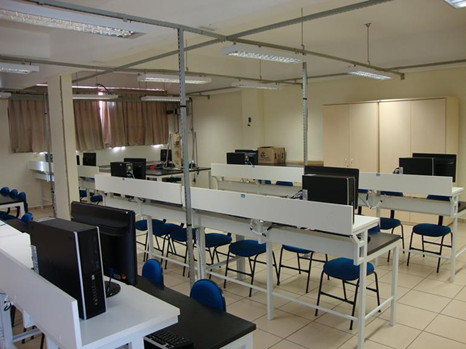
\includegraphics[width=0.85\textwidth]{Caps/Figs/lab004a.png}
    \fonte{\utf}
    \label{fig:lab004a}
\end{figure}

\begin{figure}[!htb]
    \centering
    \caption{Visão anterior do Laboratório de Sistemas Digitais}
    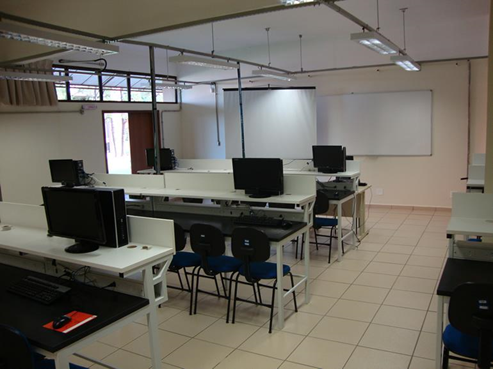
\includegraphics[width=0.85\textwidth]{Caps/Figs/lab004b.png}
    \fonte{\utf}
    \label{fig:lab004b}
\end{figure}

\begin{figure}[!htb]
    \centering
    \caption{Exemplo de equipamentos do Laboratório de Sistemas Digitais}
    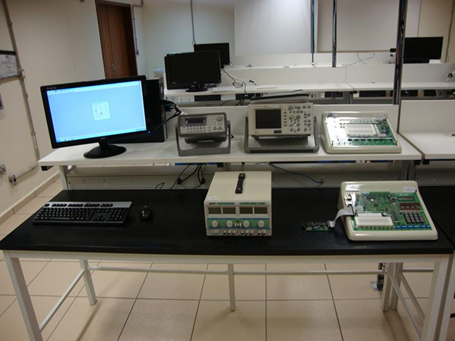
\includegraphics[width=0.85\textwidth]{Caps/Figs/lab004c.png}
    \fonte{\utf}
    \label{fig:lab004c}
\end{figure}

\subsection{Laboratório de Máquinas Elétricas}

O Laboratório de Máquinas Elétricas está localizado no Bloco A, Térreo, sala A-005.01 com 50 m\textsuperscript{2}. É equipado com:

\begin{itemize}
    \item 8 bancadas; 
    \item 3 máquinas síncronas 1 kW-1800 rpm, 60 Hz; 
    \item 3 máquinas de corrente contínua 1,25 cv / 1800 rpm; 
    \item 3 motores de rotor bobinado 1 cv-1800 rpm; 
    \item 5 motores de indução trifásicos 1 cv-60 hz-3420 rpm-220 V/380 V; 
    \item 1 motor de indução monofásico 1 cv-60 hz-3505 rpm; 
    \item 6 transformadores monofásicos 500 VA; 
    \item 5 Transformadores monofásicos 1000 VA; 
    \item 6 transformadores trifásicos de 1000 VA; 
    \item 8 transformadores monofásicos de 100 VA; 
    \item 6 alicates wattímetro; 
    \item 3 tacômetros ópticos digitais; 
    \item 3 variadores de tensão trifásicos de 2910 VA; 
    \item 3 variadores de tensão monofásicos de 1800 VA; 
    \item 3 fontes de alimentação com saída CC ajustável de 0-300 V/750 W; 
    \item 3 reostatos para controle de corrente de excitação de máquinas síncrona; 
    \item 3 reostatos de carga para controle de velocidade de motor de indução tipo rotor bobinado; 
    \item 3 resistências de carga para utilização em experiências com máquinas elétricas; e
    \item 3 fontes CC variáveis para alimentação de campo de máquinas rotativas.    
\end{itemize}

Neste laboratório são desenvolvidas atividades práticas das seguintes disciplinas do curso:

\begin{itemize}
    \item Conversão de Energia 1;
    \item Máquinas e Acionamentos.    
\end{itemize}

O ambiente do laboratório e exemplos dos modelos de equipamentos disponíveis aos alunos são apresentados na Figura 5, Figura 6 e Figura 7.

\begin{figure}[!htb]
    \centering
    \caption{Visão do Laboratório de Máquinas Elétricas}
    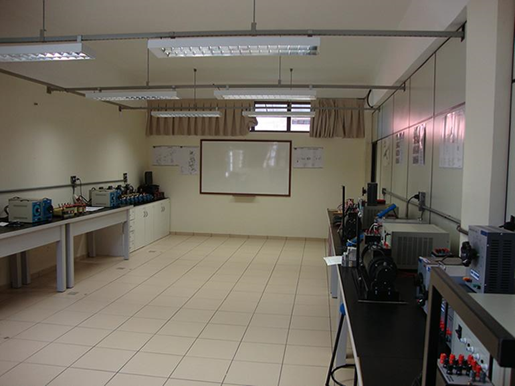
\includegraphics[width=0.85\textwidth]{Caps/Figs/lab005.01a.png}
    \fonte{\utf}
    \label{fig:lab005.01a}
\end{figure}

\begin{figure}[!htb]
    \centering
    \caption{Exemplo de equipamentos do Lab. Máquinas Elétricas}
    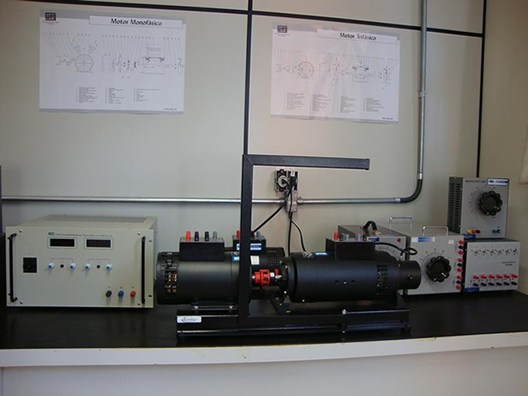
\includegraphics[width=0.85\textwidth]{Caps/Figs/lab005.01b.png}
    \fonte{\utf}
    \label{fig:lab005.01b}
\end{figure}

\begin{figure}[!htb]
    \centering
    \caption{Exemplo de equipamentos do Lab. Máquinas Elétricas}
    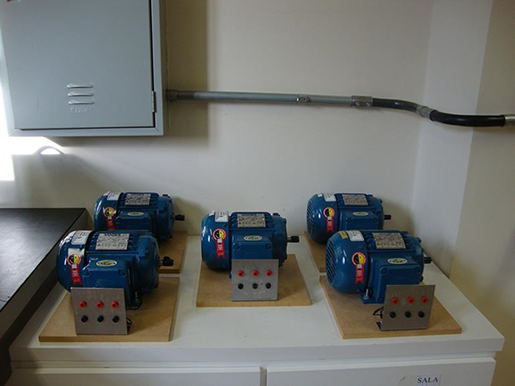
\includegraphics[width=0.85\textwidth]{Caps/Figs/lab005.01c.png}
    \fonte{\utf}
    \label{fig:lab005.01c}
\end{figure}

\subsection{Laboratório de Instalações Elétricas}

O Laboratório de Instalações Elétricas está localizado no Bloco A, Térreo, sala A-05.02 com 50 m\textsuperscript{2}. É equipado com:

\begin{itemize}
    \item 8 bancadas;
    \item 3 kits didáticos de instalações prediais; 
    \item 10 kits didáticos de medidas elétricas; 
    \item 1 analisador de qualidade de energia; 
    \item 1 terrômetro digital; 
    \item 1 medidor de resistência de isolação; 
    \item 10 transformadores de corrente 40/5 A; 
    \item 9 luxímetro digital; 
    \item 3 termômetros infravermelho; 
    \item 2 medidores de distância ultrassônico digital; 
    \item 2 multímetros digitais; 
    \item 2 medidores de campo magnético digital;
    \item 2 relógios termo-higrômetro; 
    \item 3 reostatos 0-50 W/1 A; 
    \item 1 decibelímetro; 
    \item 3 medidores RLC; 
    \item 1 alicate wattímetro; 
    \item 2 amperímetros de bancada analógicos; 
    \item 2 voltímetros de bancada analógicos; 
    \item 2 varímetros de bancada analógicos; 
    \item 2 wattímetros de bancada analógicos; 
    \item 6 reostatos linear (0-100 W); 
    \item 6 fontes DC JNG saída 24 V/14,6 A; 
    \item 5 wattímetros analógicos 0-1200 W;
    \item 5 varímetros analógicos 0-1200 VAR; 
    \item 5 amperímetros analógicos 0-5 A; e
    \item 5 voltímetros analógicos 0-250 V.    
\end{itemize}

Neste laboratório são desenvolvidas atividades práticas das seguintes disciplinas do curso:

\begin{itemize}
    \item Instalações Elétricas Prediais;
    \item Máquinas e Acionamentos;
    \item Conversão de Energia 1;e
    \item Medidas e Sensores.    
\end{itemize}

O ambiente do laboratório e exemplos dos modelos de equipamentos disponíveis aos alunos são apresentados na \autoref{fig:lab005.02a} e \autoref{fig:lab005.02b}.

\begin{figure}[!htb]
    \centering
    \caption{Visão geral do Lab. de Instalações Elétricas}
    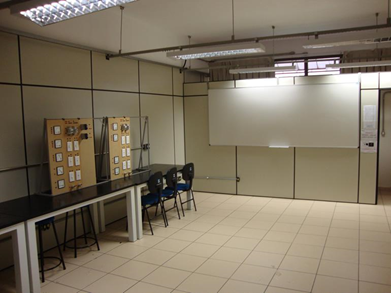
\includegraphics[width=0.85\textwidth]{Caps/Figs/lab005.02a.png}
    \fonte{\utf}
    \label{fig:lab005.02a}
\end{figure}

\begin{figure}[!htb]
    \centering
    \caption{Visão frontal do Lab. de Instalações Elétricas}
    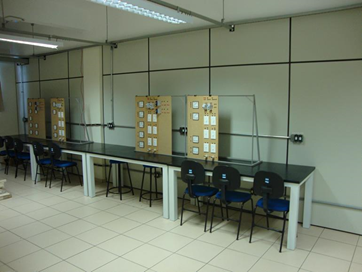
\includegraphics[width=0.85\textwidth]{Caps/Figs/lab005.02b.png}
    \fonte{\utf}
    \label{fig:lab005.02b}
\end{figure}

\subsection{Laboratório de Circuitos Elétricos}

O Laboratório de Circuitos Elétricos está localizado no Bloco A, Térreo, sala A-06 com 100,87 m\textsuperscript{2}. É equipado com:

\begin{itemize}
    \item 12 bancadas; 
    \item 12 fontes de alimentação DC; 
    \item 12 geradores de funções de 20 MHz; 
    \item 15 multímetros digitais; 
    \item 13 osciloscópios digitais de 100 MHz;
    \item 4 variac monofásico 2000 VA; e
    \item 1 variac trifásico 2000 VA.    
\end{itemize}

Neste laboratório são desenvolvidas atividades práticas das seguintes disciplinas do curso:

\begin{itemize}
    \item Circuitos Elétricos 1;
    \item Circuitos Elétricos 2;
    \item Eletrônica Analógica 1;
    \item Eletrônica Analógica 2;
    \item Eletrônica de Potência;
    \item Medidas e Sensores; e
    \item Máquinas e Equipamentos Elétricos.    
\end{itemize}

O ambiente do laboratório e exemplos dos modelos de equipamentos disponíveis aos alunos são apresentados na \autoref{fig:lab006a} e \autoref{fig:lab006b}.

\begin{figure}[!htb]
    \centering
    \caption{Visão geral do Lab. de Circuitos Elétricos}
    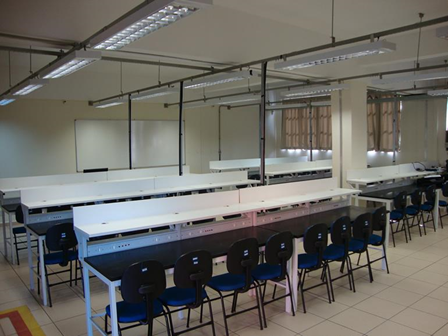
\includegraphics[width=0.85\textwidth]{Caps/Figs/lab006a.png}
    \fonte{\utf}
    \label{fig:lab006a}
\end{figure}

\begin{figure}[!htb]
    \centering
    \caption{Exemplo de equipamentos do Lab. de Circuitos Elétricos}
    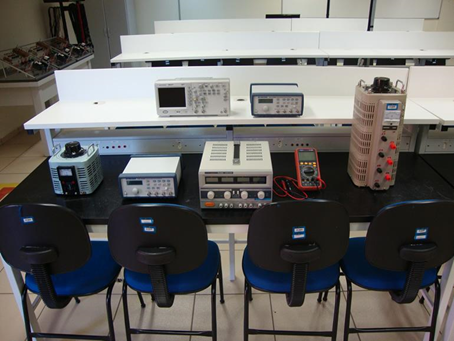
\includegraphics[width=0.85\textwidth]{Caps/Figs/lab006b.png}
    \fonte{\utf}
    \label{fig:lab006b}
\end{figure}


\subsection{Laboratório de Iniciação Científica}

O Laboratório de Iniciação Científica está localizado no Bloco A, Térreo, sala A-07.02 com 49 m\textsuperscript{2}. É equipado com:

\begin{itemize}
    \item 6 bancadas e cadeiras; 
    \item 4 armários; 
    \item 4 Computadores desktop (1x 2,5 GHz, 8 GB, 250 GB SATA);
    \item 2 Fontes de alimentação simétrica, modelo PS-5000 (ICEL);
    \item 2 Osciloscópios digital, modelo DSO1012A (Agilent);
    \item 2 Geradores de função, modelo 4040DDS (BK Precision);
    \item 2 Multímetros;
    \item 10 Kits de desenvolvimento Cypress FM4-176L-S6E2CC-ETH – ARM® Cortex®-M4 MCU Starter Kit with Ethernet and USB Host;
    \item 25	Licença para uso da plataforma Keil MDK Professional; e
    \item 2	 Kits de desenvolvimento Microchip Curiosity PIC32MZEF with Audio Daughter Card.    
\end{itemize}

Neste laboratório são desenvolvidas com prioridade às atividades práticas das seguintes disciplinas do curso:

Neste laboratório são desenvolvidas com prioridade às atividades práticas das seguintes disciplinas do curso:

\begin{itemize}
    \item TCC 1;
    \item TCC 2; e
    \item Iniciação Científica.    
\end{itemize}

Adicionalmente, o laboratório também atende as atividades de Iniciação Científica e Tecnológica, assim como as atividades extraclasse das disciplinas do curso.

O ambiente do laboratório e exemplos dos modelos de equipamentos disponíveis aos alunos são apresentados na \ref{fig:lab007.01a}, \ref{fig:lab007.01b} e \ref{fig:lab007.01b}.

\begin{figure}[!htb]
    \centering
    \caption{Vista frontal do Lab. de Iniciação Científica}
    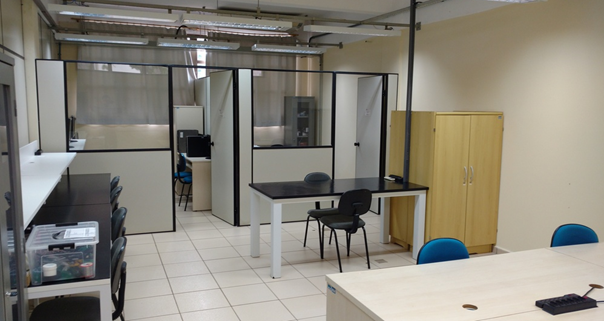
\includegraphics[width=0.85\textwidth]{Caps/Figs/lab007.01a.png}
    \fonte{\utf}
    \label{fig:lab007.01a}
\end{figure}

\begin{figure}[!htb]
    \centering
    \caption{Vista lateral do Lab. de Iniciação Científica}
    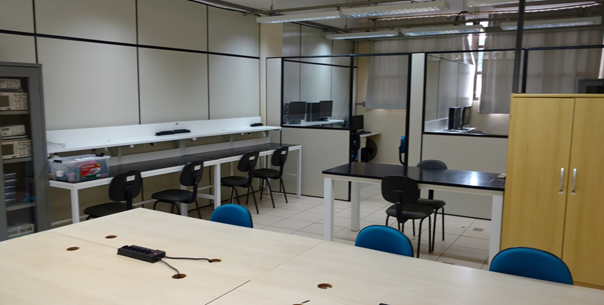
\includegraphics[width=0.85\textwidth]{Caps/Figs/lab007.01b.png}
    \fonte{\utf}
    \label{fig:lab007.01b}
\end{figure}

\begin{figure}[!htb]
    \centering
    \caption{Vista anterior do Lab. de Iniciação Científica}
    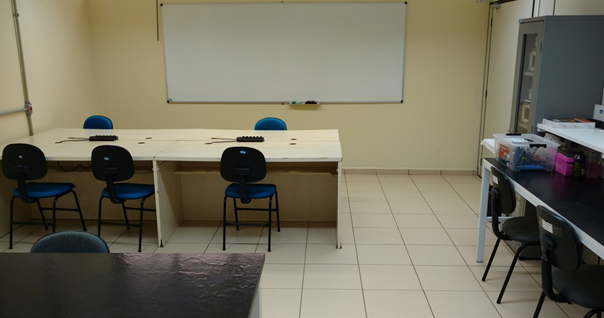
\includegraphics[width=0.85\textwidth]{Caps/Figs/lab007.01c.png}
    \fonte{\utf}
    \label{fig:lab007.01c}
\end{figure}

\subsection{Sala de Apoio Técnico / Almoxarifado}

A sala de Apoio Técnico está localizada no Bloco A, Térreo, sala A-07.01 com 38 m\textsuperscript{2}. É equipado com:

\begin{itemize}
    \item 3 bancadas; 
    \item 1 Furadeira de bancada; 
    \item 1 Carrinho de ferramentas com 6 gavetas; 
    \item 1 Sistema de confecção de protótipos de circuito impresso por método de fresagem; 
    \item 1 Forno elétrico; 
    \item 1 Furadeira elétrica manual; 
    \item 1 Serra tico-tico manual; 
    \item 1 Serra circular manual; 
    \item 1 Parafusadeira elétrica manual; e
    \item Ferramentas diversas.    
\end{itemize}



\subsection{Laboratório de Acionamentos/Controle e Automação}

O Laboratório de Acionamentos/Controle e Automação está localizado no Bloco A, Térreo, sala A-08 com 99 m\textsuperscript{2}. É equipado com:

\begin{itemize}
    \item 9 PCs com acesso à Internet; 
    \item 8 Conjuntos de CLPs; 
    \item 15 inversores de Frequência Trifásicos; 
    \item 5 Soft Starters; 8 bancadas; 
    \item 4 kits didáticos de acionamentos eletromagnéticos; 
    \item 20 motores de indução trifásicos; 
    \item 4 motores de indução monofásicos; e 
    \item 6 kits de controle.    
\end{itemize}

Neste laboratório são desenvolvidas atividades práticas das seguintes disciplinas do curso:

\begin{itemize}
    \item Controle de Sistemas Lineares 1;
    \item Controle de Sistemas Lineares 2;
    \item Controle Supervisório; e
    \item Máquinas e Acionamentos.
    
\end{itemize}

O ambiente do laboratório e exemplos dos modelos de equipamentos disponíveis aos alunos são apresentados na \autoref{fig:lab008a}, \autoref{fig:lab008b} e \autoref{fig:lab008c}.

\begin{figure}[!htb]
    \centering
    \caption{Visão geral do Lab. de Acionamentos/Controle e Automação}
    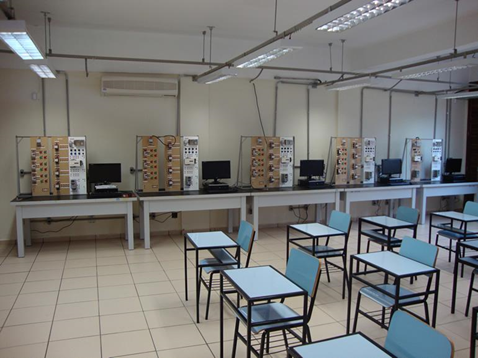
\includegraphics[width=0.85\textwidth]{Caps/Figs/lab008a.png}
    \fonte{\utf}
    \label{fig:lab008a}
\end{figure}

\begin{figure}[!htb]
    \centering
    \caption{Visão anterior do Lab. de Acionamentos/Controle e Automação}
    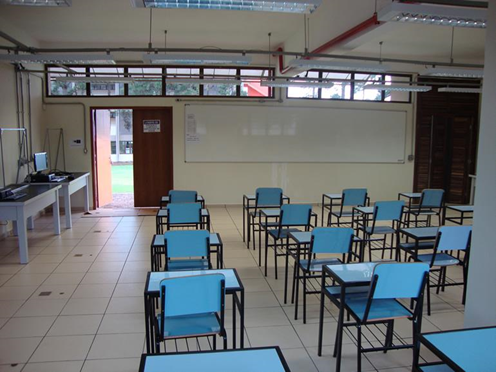
\includegraphics[width=0.85\textwidth]{Caps/Figs/lab008b.png}
    \fonte{\utf}
    \label{fig:lab008b}
\end{figure}

\begin{figure}[!htb]
    \centering
    \caption{Exemplo de equipamentos do Lab. de Acionamentos/Controle e Automação}
    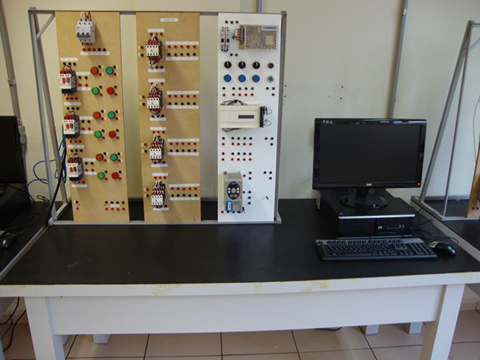
\includegraphics[width=0.85\textwidth]{Caps/Figs/lab008c.png}
    \fonte{\utf}
    \label{fig:lab008c}
\end{figure}